% Lucrare de licență — TriSense — VARIANTA COMPACTĂ
%
% Această variantă respectă recomandarea ghidului FMI de maximum 20 de pagini
% pentru capitolele IV-VII (Introducere -> Concluzii). Materialul detaliat
% (catalogul complet al jocurilor, listările de cod, figurile secundare și
% măsurile fine de robustețe) este mutat în Anexe, care nu intră în limită.
%
% Compilare: XeLaTeX (necesar pentru fontspec + polyglossia).

\documentclass[12pt, a4paper]{report}

% Suport pentru diacritice și alte simboluri
\usepackage{fontspec}

% Font Times New Roman (font real, prin fontspec)
\setmainfont{Times New Roman}

% Suport pentru mai multe limbi
\usepackage{polyglossia}

% Setează limba textului la română
\setdefaultlanguage{romanian}
% Engleză pentru rezumat
\setotherlanguages{english}

% Indentează și primul paragraf al fiecărei noi secțiuni
\SetLanguageKeys{romanian}{indentfirst=true}

% Suport pentru diferite stiluri de ghilimele
\usepackage{csquotes}

\DeclareQuoteStyle{romanian}
  {\quotedblbase}
  {\textquotedblright}
  {\guillemotleft}
  {\guillemotright}

% Utilizează biblatex pentru referințe bibliografice
\usepackage[
    maxbibnames=50,
    sorting=nty
]{biblatex}

\addbibresource{bibliography.bib}

% Spațiere inter-linie (1.5 rânduri, conform ghidului de redactare)
\usepackage{setspace}
\onehalfspacing

% Geometria paginii (margini de 2,5 cm)
\usepackage[margin=2.5cm]{geometry}

% Permite o ușoară întindere a spațiilor pentru a evita liniile care ies în margine
\setlength{\emergencystretch}{2em}

% Despărțire în silabe: hardware → hard-ware (nu har-dware)
\hyphenation{hard-ware}

% Coloane de tabel cu lățime fixă și aliniere personalizată
\usepackage{array}

% Funcții de grafică
\usepackage{graphicx}
% Încarcă imaginile din directorul `images`
\graphicspath{{./images/}}

% Diagrame desenate nativ în LaTeX
\usepackage{tikz}
\usetikzlibrary{positioning, arrows.meta, fit, backgrounds, calc}

% Listări de cod
\usepackage{listings}
\usepackage{xcolor}
\lstset{
    basicstyle=\ttfamily\small,
    breaklines=true,
    frame=single,
    numbers=left,
    numberstyle=\tiny,
    keywordstyle=\bfseries,
    commentstyle=\color{gray},
    showstringspaces=false,
    tabsize=4
}

% Linkuri interactive în PDF
\usepackage[
    colorlinks,
    linkcolor={black},
    menucolor={black},
    citecolor={black},
    urlcolor={blue}
]{hyperref}
\hypersetup{
    pdftitle={TriSense: sistem cyber-fizic adaptiv pentru robotica asistivă în intervenții pentru copii neurodivergenți},
    pdfauthor={Boca Bogdan-Nicolae},
    pdfsubject={Proiect de diplomă},
    pdfkeywords={robotică asistivă, sisteme cyber-fizice, neurodivergență, LEGO-Based Therapy}
}

% Simboluri matematice codificate Unicode
\usepackage[warnings-off={mathtools-colon,mathtools-overbracket}]{unicode-math}

% Comenzi matematice
\usepackage{amsmath}
\usepackage{mathtools}

% Formule matematice
\newcommand{\bigO}[1]{\symcal{O}\left(#1\right)}
\DeclarePairedDelimiter\abs{\lvert}{\rvert}

% Suport pentru rezumat în două limbi
\newenvironment{abstractpage}
  {\cleardoublepage\vspace*{\fill}\thispagestyle{empty}}
  {\vfill\cleardoublepage}
\renewenvironment{abstract}[1]
  {\bigskip\selectlanguage{#1}%
   \begin{center}\bfseries\abstractname\end{center}}
  {\par\bigskip}

% Suport pentru anexe
\usepackage{appendix}

% Stiluri diferite de headere și footere
\usepackage{fancyhdr}

% Legende de figuri/tabele
\usepackage{caption}
\captionsetup{
    labelfont=bf,
    font=small,
    margin=10pt,
    skip=10pt,
    justification=justified,
    singlelinecheck=false
}

% Titluri de capitole și secțiuni stilizate
\usepackage{titlesec}

% Capitolele nu încep pe pagină nouă (cerință a ghidului de redactare FMI):
% transformăm clasa „chapter” în una care curge în pagină, ca o secțiune.
\titleclass{\chapter}{straight}

% Capitol: eticheta „Capitolul N” sus, titlul mare, linie groasă dedesubt
\titleformat{\chapter}[display]
  {\normalfont\bfseries}
  {\Large\MakeUppercase{\chaptertitlename}\ \thechapter}
  {8pt}
  {\huge}
  [\vspace{6pt}{\titlerule[1.5pt]}]
\titlespacing*{\chapter}{0pt}{18pt}{20pt}

% Secțiune: îngroșată, subliniată cu o linie fină
\titleformat{\section}
  {\normalfont\Large\bfseries}
  {\thesection}{1em}{}
  [\vspace{2pt}{\titlerule[0.5pt]}]

% Subsecțiune: îngroșată, fără linie
\titleformat{\subsection}
  {\normalfont\large\bfseries}
  {\thesubsection}{1em}{}

% Metadate
\title{TriSense: sistem cyber-fizic adaptiv pentru robotica asistivă în intervenții pentru copii neurodivergenți}
\author{Boca Bogdan-Nicolae}

% Generează variabilele cu @
\makeatletter

\begin{document}

% Front matter
\cleardoublepage
\let\ps@plain

% Pagina de titlu
\begin{titlepage}

% Redu marginile pentru ca pagina de titlu să încapă pe o singură pagină.
\newgeometry{left=2cm,right=2cm,top=1.2cm,bottom=1cm}
\enlargethispage{1.5cm}

\begin{figure}[!htb]
    \centering
    \begin{minipage}{0.2\textwidth}
        
\includegraphics[width=\linewidth]{logo-ub.png}
    \end{minipage}
    \begin{minipage}{0.5\textwidth}
        \large
        \vspace{0.2cm}
        \begin{center}
            \textbf{UNIVERSITATEA DIN BUCUREȘTI}
        \end{center}
        \vspace{0.3cm}
        \begin{center}
            \textbf{
                FACULTATEA DE \\
                MATEMATICĂ ȘI INFORMATICĂ
            }
        \end{center}
    \end{minipage}
    \begin{minipage}{0.2\textwidth}
        
\includegraphics[width=\linewidth]{logo-fmi.png}
    \end{minipage}
\end{figure}

\begin{center}
\textbf{SPECIALIZAREA TEHNOLOGIA INFORMAȚIEI}
\end{center}

\vspace{0.55cm}

\begin{center}
\Large \textbf{Proiect de diplomă}
\end{center}

\begin{center}
\LARGE \textbf{\MakeUppercase{TriSense: sistem cyber-fizic adaptiv pentru robotica asistivă în intervenții pentru copii neurodivergenți}}
\end{center}

\vspace{1.25cm}

\begin{center}
\large \textbf{Absolvent \\ \@author}
\end{center}

\vspace{0.2cm}

\begin{center}
\large \textbf{Coordonator științific \\ Lect. Dr. Anca Dobrovăț}
\end{center}

\vfill

\begin{center}
\Large \textbf{București, iunie 2026}
\end{center}
\end{titlepage}

\restoregeometry
\newgeometry{
    margin=2.5cm
}

\fancypagestyle{main}{
  \fancyhf{}
  \renewcommand\headrulewidth{0.4pt}
  \fancyhead[L]{\small\itshape\nouppercase{\leftmark}}
  \fancyhead[R]{\small TriSense}
  \fancyfoot[C]{\thepage}
}

\addtocounter{page}{1}

% Rezumatul
\begin{abstractpage}

\begin{abstract}{romanian}
Lucrarea de față prezintă proiectarea, implementarea și evaluarea sistemului \textbf{TriSense}, un sistem cyber-fizic adaptiv destinat roboticii asistive în intervențiile pentru copii neurodivergenți. TriSense integrează trei niveluri de execuție interconectate: un robot construit pe platforma LEGO\textsuperscript{®} SPIKE\texttrademark{} Prime (firmware Pybricks), o placă LMS-ESP32 cu MicroPython responsabilă de comunicație și audio, și o aplicație de tip „creier” care rulează pe PC, scrisă în Python. Comunicarea între componente folosește protocolul MQTT, un canal serial LPF2 între hub și ESP32, precum și fluxuri audio PCM prin TCP. Componenta de inteligență artificială se bazează pe modelele Google Gemini pentru dialog, transcrierea vorbirii și analiza vizuală a construcțiilor LEGO realizate de copil, capturate cu un modul ESP32-CAM. Sistemul oferă un set de activități terapeutice interactive — recunoașterea emoțiilor, imitarea tiparelor de mișcare, jocul de construcție „Build the Model” inspirat de Turnul din Hanoi, jocuri de funcții executive (Stop \& Go, estimarea timpului), o poveste co-construită și exerciții de respirație pentru autoreglare emoțională — împreună cu înregistrarea automată de metrici de sesiune utile terapeuților. Rezultatele obținute arată că o arhitectură distribuită, construită din componente accesibile, poate susține interacțiuni multimodale (voce, mișcare, vedere artificială) adaptate nevoilor copiilor neurodivergenți.
\end{abstract}

\begin{abstract}{english}
This thesis presents the design, implementation and evaluation of \textbf{TriSense}, an adaptive cyber-physical system for assistive robotics in interventions for neurodivergent children. TriSense integrates three interconnected execution levels: a robot built on the LEGO\textsuperscript{®} SPIKE\texttrademark{} Prime platform (Pybricks firmware), an LMS-ESP32 board running MicroPython that handles communication and audio, and a Python ``brain'' application running on a PC. The components communicate through the MQTT protocol, an LPF2 serial channel between the hub and the ESP32, and PCM audio streams over TCP. The artificial-intelligence component relies on Google Gemini models for dialogue, speech transcription and visual analysis of the LEGO constructions built by the child, captured with an ESP32-CAM module. The system offers a set of interactive therapeutic activities --- emotion recognition, movement-pattern imitation, the ``Build the Model'' construction game inspired by the Tower of Hanoi, executive-function games (Stop \& Go, time estimation), a co-constructed story, and breathing exercises for emotional self-regulation --- together with the automatic logging of session metrics useful to therapists. The results show that a distributed architecture, built from affordable components, can support multimodal interactions (voice, movement, computer vision) tailored to the needs of neurodivergent children.
\end{abstract}

\end{abstractpage}


\tableofcontents

% Main matter
\cleardoublepage
\pagestyle{main}
\let\ps@plain\ps@main

\chapter{Introducere}
\label{cap:introducere}

\section{Context și motivație}

Aproximativ unul din 36 de copii primește astăzi un diagnostic din spectrul autist, iar prevalența ADHD în populația pediatrică depășește 5\%. În spatele acestor cifre stau familii care caută intervenții timpurii, terapeuți supraîncărcați și — în România în mod special — un decalaj considerabil între nevoia de servicii specializate și disponibilitatea lor. Orice instrument care poate extinde capacitatea unui terapeut, fără a-i lua locul, are așadar o miză practică reală.

Două direcții de cercetare, dezvoltate independent, sugerează o astfel de oportunitate. Prima este terapia bazată pe LEGO (LEGO-Based Therapy), formalizată de dr. Daniel LeGoff \cite{legoff2004} pornind de la o observație simplă: copiii cu autism, care evită de regulă interacțiunile sociale, colaborează spontan atunci când mediul de joc este un set de piese LEGO — un sistem cu reguli fizice clare, predictibil și lipsit de ambiguitatea care face interacțiunea umană obositoare pentru ei. Studiile ulterioare \cite{legoff2006, owens2008} au confirmat că abilitățile sociale exersate în acest cadru se mențin și se transferă. A doua direcție este robotica asistivă: o literatură consistentă \cite{scassellati2012, robins2005, cabibihan2013} documentează un fenomen aparent paradoxal — mulți copii cu autism interacționează mai ușor cu roboții decât cu oamenii, fiindcă robotul este predictibil, răbdător și nu transmite semnale sociale contradictorii. Mai mult, studii precum cel al lui Kim și colaboratorii \cite{kim2013} arată că prezența robotului crește interacțiunea copilului \emph{cu adulții din încăpere}: robotul funcționează ca mediator social, nu ca substitut.

Legătura cu practica nu a rămas doar teoretică. În timpul dezvoltării proiectului am avut ocazia să lucrez alături de psihoterapeuții Marius și Andreea Lumpan, în cadrul primei inițiative de LEGO-Based Therapy din România dedicată copiilor neurodivergenți \cite{lumpanagerpres2025}. Experiența lor mi-a permis să observ direct cum interacționează copiii cu materialul LEGO în context terapeutic — colaborarea, toleranța la frustrare, ritmul sesiunii, rolul adultului care intervine înainte de escaladare. Aceste observații au influențat direct deciziile de design ale TriSense: instrucțiuni scurte, feedback fără penalizare, ritualuri predictibile și pauze de reglare.

TriSense s-a născut la intersecția acestor două direcții. L-am pornit ca proiect personal pentru competiția World Robot Olympiad (categoria Proiect), iar în cadrul acestei lucrări l-am dezvoltat într-un sistem complet — întreaga construcție, de la hardware la cod, fiind realizată individual. Întrebarea de la care am plecat a fost pragmatică: se poate construi, din componente accesibile oricărei școli sau cabinet — un set LEGO educațional, două plăci de dezvoltare de câteva zeci de lei și un laptop obișnuit — un robot capabil să susțină activități terapeutice reale, cu dialog vocal, jocuri structurate și feedback obiectiv pentru terapeut?

\section{Problema abordată}

Formulată tehnic, problema centrală a lucrării este \emph{proiectarea și implementarea unui sistem cyber-fizic care să orchestreze, în timp real și fiabil, componente diferite — un hub LEGO cu resurse minimale, un microcontroler cu Wi-Fi, o cameră independentă și servicii de inteligență artificială în cloud — într-o experiență de interacțiune coerentă, predictibilă și adaptată copiilor neurodivergenți.} Dificultatea nu stă în niciuna dintre componente luată separat, ci în integrarea lor: hub-ul LEGO nu are rețea, placa ESP32 are rețea dar resurse de calcul limitate, iar modelele de inteligență artificială rulează în cloud, cu latențe variabile — în timp ce utilizatorul final este un copil pentru care orice întrerupere sau comportament imprevizibil poate compromite sesiunea.

\section{Obiectivele și contribuțiile lucrării}

Obiectivul general este realizarea unui sistem robotic asistiv funcțional cap-coadă, validat pe hardware real. Din el decurg obiectivele specifice și, totodată, principalele contribuții — de natură implementativă, întrucât sistemul există, funcționează și a fost testat pe hardware real:

\begin{itemize}
    \item o \textbf{arhitectură distribuită pe trei niveluri} (hub LEGO cu Pybricks, placă LMS-ESP32 cu MicroPython, aplicație Python pe PC), cu protocoale adecvate fiecărui tip de trafic: MQTT pentru control, canal serial LPF2 pentru legătura hub--ESP32 și fluxuri TCP pentru audio;
    \item un \textbf{lanț vocal complet} — captură audio pe robot, transcriere automată, generarea răspunsului cu un model de limbaj și sinteză vocală redată pe difuzor — cu latență și calitate acceptabile pentru un dialog natural;
    \item un \textbf{canal bidirecțional} peste LPF2 care transmite și apăsările butoanelor fizice ale hub-ului, transformând robotul într-o interfață de intrare pentru copil;
    \item un \textbf{set de activități terapeutice} inspirate din literatura de specialitate: recunoașterea emoțiilor, imitarea tiparelor de mișcare, jocul de construcție „Build the Model” cu verificare vizuală, exercițiul de respirație, jocuri de funcții executive (Stop \& Go, estimarea timpului, categorii rapide), povestea co-construită și o rutină de dans;
    \item o \textbf{metodă de verificare a construcțiilor LEGO} bazată pe descrieri în limbaj natural și un model multimodal zero-shot, cu prag calibrat empiric, extensibilă fără date de antrenare;
    \item \textbf{colectarea automată a metricilor de sesiune} (activități, durate, încercări, reușite) într-un format direct utilizabil de terapeut.
\end{itemize}

\section{Structura lucrării}

Capitolul~\ref{cap:preliminarii} parcurge fundamentele teoretice și studiile de specialitate, inclusiv poziționarea față de orientările psihologice majore. Capitolul~\ref{cap:arhitectura} prezintă arhitectura sistemului și fluxurile de date. Capitolul~\ref{cap:implementare} coboară la nivelul implementării — firmware, aplicația de pe PC, jocurile și componenta de viziune — materialul detaliat fiind reluat în anexe. Capitolul~\ref{cap:evaluare} descrie testarea, rezultatele și considerațiile etice, iar capitolul~\ref{cap:concluzii} sintetizează concluziile și direcțiile de dezvoltare. Anexa~\ref{anexa:cod} prezintă structura proiectului software; catalogul detaliat al jocurilor și fragmentele de cod sunt în anexa~\ref{an:cap:implementare}.

\chapter{Fundamente teoretice și studii de specialitate}
\label{cap:preliminarii}

Acest capitol trece în revistă literatura care a stat la baza proiectului: studiile clinice despre terapia bazată pe LEGO și despre interacțiunea copiilor cu autism cu roboții, reperele constructiviste și socioculturale, poziționarea eclectică față de orientările psihologice majore și, în final, conceptele și tehnologiile pe care se sprijină implementarea.

\section{Neurodivergența, suprasolicitarea senzorială și funcțiile executive}
\label{sec:meltdown}

Termenul de \emph{neurodivergență} descrie variațiile naturale ale funcționării neurologice umane — tulburările din spectrul autist (TSA), ADHD, dislexia ș.a. Conform DSM-5 \cite{apa2013}, TSA se caracterizează prin deficite persistente în comunicarea și interacțiunea socială, alături de tipare restrictive și repetitive de comportament. Pentru lucrarea de față, două aspecte sunt esențiale: copiii din spectru procesează cu dificultate indiciile sociale subtile (expresii, ton, contact vizual), ceea ce face interacțiunea umană obositoare, dar răspund foarte bine la medii \emph{structurate și predictibile} — ambele observații conduc direct către robotică. În cazul ADHD, dificultățile centrale țin de funcțiile executive — control inhibitor, memorie de lucru și flexibilitate cognitivă \cite{diamond2013} — funcții pe care Diamond arată că le putem antrena prin exerciții repetate, gradate ca dificultate, exact tipul de activitate pe care un sistem robotic îl administrează cu o consecvență pe care un om nu o poate garanta sesiune după sesiune.

Un fenomen central pentru orice intervenție este criza de suprasolicitare (\emph{meltdown}), distinctă de capriciu: nu este un comportament orientat spre un scop, ci o reacție involuntară de descărcare, declanșată când acumularea de stimuli depășește capacitatea de procesare a copilului. Mazefsky și colaboratorii \cite{mazefsky2013} arată că dificultățile de reglare emoțională sunt un mecanism central al TSA, iar relatările adolescenților autiști culese de Phung și colaboratorii \cite{phung2021} confirmă două concluzii practice: episoadele pot fi adesea \emph{prevenite} dacă semnele timpurii sunt observate la timp, iar reacția cea mai utilă este una calmă, predictibilă și lipsită de judecată. Aceste observații au modelat TriSense pe plan preventiv (structură predictibilă, feedback pozitiv, exercițiu de respirație) și educativ (robotul poate interpreta o variantă stilizată și inofensivă a stării de criză, după care „se liniștește” prin propria rutină de respirație, oferind copilului ocazia de a observa și denumi starea din exterior).

\section{Terapia bazată pe LEGO}

Punctul de plecare conceptual al proiectului este terapia bazată pe LEGO (LBT), formalizată de doctorul Daniel LeGoff pornind de la o observație din sala de așteptare: doi copii cu autism, care nu inițiau interacțiuni sociale, au început spontan să vorbească despre construcțiile lor LEGO \cite{legoff2004}. În studiul inițial pe 47 de copii, urmăriți 24 de săptămâni, LeGoff a măsurat îmbunătățiri pe trei dimensiuni — frecvența autoinițierii contactului social, durata interacțiunilor și reducerea comportamentelor stereotipe — iar un follow-up pe trei ani \cite{legoff2006} a confirmat că efectele se mențin. Independent, grupul lui Baron-Cohen de la Cambridge a comparat LBT cu un alt program de abilități sociale și a găsit ameliorări superioare în grupul LEGO \cite{owens2008}, atribuite caracterului \emph{intrinsec motivant} al materialului: copiii nu „fac terapie”, ci se joacă, iar abilitățile sociale se exersează ca efect secundar. Sistemul LEGO funcționează tocmai pentru că este predictibil — piesele se îmbină într-un singur mod corect, regulile sunt fizice, nu sociale — iar construcția după model implică planificare, memorie de lucru și persistență la sarcină. TriSense preia acest cadru și îl augmentează: robotul devine partenerul de joc care propune modelul, urmărește construcția și oferă feedback. În România, metoda a fost adaptată de psihoterapeuții Marius și Andreea Lumpan \cite{lumpanagerpres2025}, iar experiența mea alături de ei a completat lectura articolelor: am observat direct cum terapeutul calibrează ritmul sesiunii și când intervine înainte de escaladare.

\section{Repere psihologice: constructivism, învățare socioculturală și orientări majore}

Designul activităților se sprijină pe constructivismul lui Piaget și pe teoria socioculturală a lui Vygotsky. Piaget descrie dezvoltarea ca proces activ: copilul își construiește înțelegerea prin acțiune asupra mediului \cite{piaget1969}; manipularea pieselor LEGO este învățare prin acțiune — copilul formulează o ipoteză, o testează, primește feedback și ajustează. Vygotsky mută accentul pe \emph{medierea socială}: învățarea apare în zona proximală de dezvoltare, unde un partener mai competent structurează sarcina și retrage treptat ajutorul \cite{vygotsky1978}. TriSense se plasează ca \emph{mediator} — nu înlocuiește terapeutul, dar oferă scaffolding consecvent: instrucțiuni scurte, același ritual, feedback fără pedeapsă, dificultate crescătoare.

Proiectul este deliberat eclectic față de cele trei mari orientări istorice ale psihologiei. Jocurile care antrenează funcțiile executive (Stop \& Go, construcții gradate, fluență semantică) urmează logica \emph{cognitiv-comportamentală}: practică repetată, feedback imediat, întărire pozitivă \cite{diamond2013}. În schimb, modul de a aborda meltdown-ul urmează o orientare \emph{umanistă}: Rogers descrie relația terapeutică drept cadru de acceptare necondiționată, în care persoana nu este redusă la un set de comportamente corectabile \cite{rogers1951} — de aceea robotul nu „sancționează” eșecul, iar scenariile de criză sunt stilizate, voluntare și urmate de reglare, sub supravegherea unui adult. Această complementaritate este o alegere de design: robotul aduce consistența exercițiilor structurate; terapeutul uman aduce empatia, intuiția și decizia de oprire — el observă semnele de suprasolicitare pe care robotul nu le \emph{simte}. Definirea activităților și a constrângerilor etice a fost discutată cu Marius și Andreea Lumpan \cite{lumpanagerpres2025}, nu ca validare clinică, ci ca verificare că jocurile rămân blânde și utile într-un context ghidat de adult. Un ultim reper vine din metoda \emph{Social Stories} a lui Carol Gray \cite{gray2010}: scenarii sociale scurte, formulate identic la fiecare repetare — principiu pe care TriSense îl aplică în salutul, formulele de încurajare și ritualul de încheiere.

\section{Robotica asistivă în intervențiile pentru copii cu autism}

Dacă dificultățile copiilor cu TSA sunt sociale, de ce am introduce o mașină? Pentru că interacțiunea umană este copleșitoare informațional, în timp ce un robot este \emph{simplu, predictibil și răbdător}. Dautenhahn și Werry, pionierii proiectului AURORA, au argumentat încă din 2004 că tocmai această simplitate controlabilă face din robot un mediator ideal — un pas intermediar între lumea predictibilă a obiectelor și cea impredictibilă a oamenilor \cite{dautenhahn2004}. Sintezele ulterioare confirmă: Scassellati, Admoni și Matarić \cite{scassellati2012} documentează că în prezența roboților copiii cu TSA manifestă contact vizual prelungit, atenție comună, imitație spontană și inițierea interacțiunii, comportamente care se extind și către adulții prezenți; Robins și colaboratorii \cite{robins2005}, cu robotul KASPAR, arată că robotul funcționează ca \emph{mediator social}; iar Kim și colaboratorii \cite{kim2013} găsesc că un copil cu TSA vorbește mai mult cu un adult în prezența unui robot. Sintezele critice impun și prudență — eșantioane mici, design exploratoriu \cite{diehl2012, pennisi2016} — iar Cabibihan și colaboratorii \cite{cabibihan2013} și Ricks și Colton \cite{ricks2010} observă că roboții non-umanoizi sunt adesea mai bine primiți decât cei cu aspect uman realist. Poziționarea TriSense este directă: un robot non-umanoid din piese LEGO, partener de joc și mediator, care administrează activități inspirate din LBT și din probele de funcții executive și produce metrici obiective — fără nicio pretenție de diagnostic.

Mai multe jocuri sunt inspirate din probe consacrate în neuropsihologie, adaptate ludic: „Build the Model” pornește de la \emph{Turnul din Hanoi} (planificare vizuo-spațială), „Stop \& Go” de la paradigma Go/No-Go (control inhibitor), estimarea timpului de la probele de percepție temporală, iar „categoriile rapide” de la fluența semantică. Statutul lor este însă explicit: sunt \emph{exerciții inspirate din procedee standard, nu teste clinice validate} — TriSense nu măsoară inteligența și nu diagnostichează.

\section{Sisteme cyber-fizice și tehnologiile utilizate}

Un \emph{sistem cyber-fizic} (CPS) integrează strâns calculul, comunicația și procesele fizice, cu o componentă de calcul adesea distribuită, în buclă închisă cu mediul \cite{lee2008}. Lee subliniază că provocarea centrală nu este puterea de calcul, ci \emph{orchestrarea}: sincronizarea în timp real a unor componente cu cerințe de fiabilitate pe care software-ul de birou nu le are. TriSense este un CPS în sens deplin — percepe vocea (microfon), construcția (cameră) și apăsările de buton, le procesează printr-o componentă distribuită pe trei dispozitive plus servicii cloud și le transformă în acțiuni fizice (mișcări, animații pe LED-uri, vorbire), caracterul adaptiv venind din stratul de inteligență artificială.

Pe partea hardware, robotul folosește platforma \textbf{LEGO\textsuperscript{®} SPIKE\texttrademark{} Prime} cu firmware-ul open-source \emph{Pybricks} \cite{pybricks}, ales pentru controlul fin al motoarelor și matricei de LED-uri și pentru accesul programabil la portul LPF2. Placa \textbf{LMS-ESP32} \cite{antonsmindstorms} se conectează la acest port și aduce ce îi lipsește hub-ului — Wi-Fi, audio I2S și putere de calcul — rulând MicroPython \cite{micropython}; ea coordonează un amplificator MAX98357A cu difuzor și un microfon INMP441. Pentru viziune, un modul \textbf{ESP32-CAM} de cost redus livrează imagini JPEG la cerere prin HTTP. Comunicația folosește trei mecanisme: \textbf{MQTT} \cite{mqtt} (publish/subscribe, prin brokerul Mosquitto) pentru control, \textbf{LPF2} cu biblioteca \emph{PupRemote} \cite{pupremote} pentru legătura hub--ESP32 (canalele \texttt{cmd} și \texttt{btn}) și conexiuni \textbf{TCP} directe pentru fluxurile audio PCM. Componenta de inteligență artificială se bazează pe modelele \textbf{Google Gemini} \cite{gemini} pentru dialog (cu un \emph{system prompt} care impune un ton cald și propoziții scurte), pentru transcrierea vorbirii și pentru verificarea vizuală a construcțiilor în regim \emph{zero-shot} — modelul primește fotografia și o descriere în limbaj natural a țintei și întoarce un verdict structurat, fără date de antrenare. Sinteza vocală folosește Google Cloud TTS, cu \texttt{edge-tts} ca alternativă locală.

\chapter{Arhitectura sistemului TriSense}
\label{cap:arhitectura}

\section{Privire de ansamblu}

Forma arhitecturii a rezultat din constrângerile fiecărei componente: hub-ul LEGO are motoare și butoane, dar nu are Wi-Fi; placa ESP32 are Wi-Fi și interfață audio, dar nu poate rula modele de inteligență artificială; PC-ul poate orice, dar nu are corp. Soluția firească a fost un sistem distribuit pe trei niveluri, în care fiecare dispozitiv face exact ceea ce știe cel mai bine:

\begin{enumerate}
    \item \textbf{Nivelul fizic — hub-ul LEGO SPIKE Prime} (firmware Pybricks, \texttt{main.py}): controlează motoarele brațelor și roților, desenează animații pe matricea de LED-uri $5\times5$ și citește butoanele. Nu ia nicio decizie — primește coduri de acțiune pe canalul \texttt{cmd} și raportează butoanele pe canalul \texttt{btn}.
    \item \textbf{Nivelul de comunicație — placa LMS-ESP32} (MicroPython, \texttt{main\_robot.py}): puntea dintre lumea LEGO și rețea — menține Wi-Fi și sesiunea MQTT, traduce mesajele de control în comenzi LPF2, redă pe difuzorul I2S audio primit prin TCP și înregistrează de la microfon.
    \item \textbf{Nivelul cognitiv — aplicația de pe PC} (Python, clasa \texttt{TriSenseBrain}): aici se iau toate deciziile — stările, dialogul, transcrierea și sinteza vocală, logica jocurilor, metricile.
\end{enumerate}

Al patrulea participant este modulul \textbf{ESP32-CAM}, conectat independent la Wi-Fi, care livrează o fotografie JPEG la fiecare cerere pe endpoint-ul \texttt{/capture}. Imaginea de ansamblu este redată în figura~\ref{fig:arhitectura}.

\begin{figure}[htb]
    \centering
    \resizebox{\textwidth}{!}{%
    \begin{tikzpicture}[
        font=\small,
        bloc/.style={draw, rounded corners=2mm, align=center, minimum height=13mm, inner sep=3mm, thick},
        eticheta/.style={font=\scriptsize, align=center, fill=white, inner sep=2pt, outer sep=1pt},
        nivel/.style={draw=gray!70, dashed, rounded corners=3mm, inner sep=5mm},
        niveltext/.style={font=\scriptsize\itshape, text=gray, anchor=south west},
        sageata/.style={-{Stealth[length=2.5mm]}, semithick},
        dubla/.style={{Stealth[length=2.5mm]}-{Stealth[length=2.5mm]}, semithick},
    ]
        \node[bloc, fill=white] (copil)
            {\textbf{Copilul}\\{\scriptsize vorbește $\cdot$ apasă butoanele $\cdot$ construiește din LEGO}};
        \node[bloc, fill=yellow!45, below=12mm of copil, minimum width=68mm] (hub)
            {\textbf{Hub LEGO SPIKE Prime} (Pybricks)\\{\scriptsize motoare brațe/roți $\cdot$ matrice LED $5\times5$ $\cdot$ butoane}};
        \node[bloc, fill=teal!30, below=22mm of hub, minimum width=68mm] (lms)
            {\textbf{LMS-ESP32} (MicroPython)\\{\scriptsize Wi-Fi $\cdot$ client MQTT $\cdot$ audio I2S (difuzor + microfon)}};
        \node[bloc, fill=cyan!20, right=30mm of lms] (cam)
            {\textbf{ESP32-CAM}\\{\scriptsize server HTTP \texttt{/capture}}};
        \node[bloc, fill=red!20, below=28mm of lms] (broker)
            {\textbf{Broker MQTT}\\{\scriptsize Mosquitto}};
        \node[bloc, fill=blue!10, left=18mm of broker] (brain)
            {\textbf{TriSenseBrain}\\{\scriptsize stări $\cdot$ jocuri $\cdot$ dialog $\cdot$ metrici}};
        \node[bloc, fill=blue!10, right=18mm of broker] (bridge)
            {\textbf{Puntea de viziune}\\{\scriptsize \texttt{vision\_esp32cam\_bridge.py}}};
        \node[bloc, fill=violet!15, below=20mm of brain] (tts)
            {\textbf{Sinteză vocală}\\{\scriptsize Cloud TTS / edge-tts}};
        \node[bloc, fill=violet!15, below=20mm of broker] (gemini)
            {\textbf{Google Gemini}\\{\scriptsize dialog $\cdot$ STT $\cdot$ Vision}};
        \begin{scope}[on background layer]
            \node[nivel, fit=(hub)] (n1) {};
            \node[nivel, fit=(lms)] (n2) {};
            \node[nivel, fit=(brain)(broker)(bridge)] (n3) {};
            \node[nivel, fit=(tts)(gemini)] (n4) {};
        \end{scope}
        \node[niveltext] at (n1.north west) {Nivelul fizic};
        \node[niveltext] at (n2.north west) {Nivelul de comunicație};
        \node[niveltext] at (n3.north west) {Nivelul cognitiv — PC};
        \node[niveltext] at (n4.north west) {Servicii cloud};
        \draw[sageata] (copil) -- (hub);
        \draw[sageata] ([xshift=-15mm]hub.south) -- node[eticheta, left=2mm] {\texttt{btn}: butoane}
            ([xshift=-15mm]lms.north);
        \draw[sageata] ([xshift=15mm]lms.north) -- node[eticheta, right=2mm] {\texttt{cmd}: acțiuni}
            ([xshift=15mm]hub.south);
        \node[eticheta] at ($(hub.south)!0.5!(lms.north)$) {LPF2 / PupRemote};
        \draw[dubla] (lms) -- node[eticheta, right=2mm] {MQTT} (broker);
        \draw[dubla] (lms.south west) -- (brain.north);
        \node[eticheta, anchor=east] at ([xshift=-3mm]$(lms.south west)!0.5!(brain.north)$)
            {TCP 8765/8766\\audio PCM};
        \draw[dubla] (brain) -- node[eticheta, above] {MQTT} (broker);
        \draw[dubla] (broker) -- node[eticheta, above] {MQTT} (bridge);
        \draw[dubla] (bridge.north) -- (cam.south);
        \node[eticheta, anchor=west] at ([xshift=3mm]$(bridge.north)!0.5!(cam.south)$)
            {HTTP\\fotografie JPEG};
        \draw[sageata] (brain) -- node[eticheta, left=2mm] {text de rostit} (tts);
        \draw[sageata] (brain.south east) -- (gemini.north west);
        \node[eticheta] at ([yshift=4mm]$(brain.south east)!0.55!(gemini.north west)$)
            {transcriere $\cdot$ dialog};
        \draw[sageata] (bridge.south west) -- (gemini.north east);
        \node[eticheta] at ([yshift=4mm]$(bridge.south west)!0.55!(gemini.north east)$)
            {imagine + descriere-țintă};
    \end{tikzpicture}%
    }
    \caption{Arhitectura logică a sistemului TriSense: cele trei niveluri de execuție (hub LEGO, LMS-ESP32, PC), modulul ESP32-CAM și serviciile cloud, împreună cu protocoalele de comunicație dintre ele.}
    \label{fig:arhitectura}
\end{figure}

\section{Protocoalele de comunicație și fluxurile de date}

Nu există un protocol universal potrivit — fiecare tip de trafic are nevoi diferite, iar sistemul folosește trei mecanisme în paralel. \textbf{MQTT} transportă mesajele de control (scurte, sporadice): modelul publish/subscribe cu broker central decuplează componentele, iar mesajele \emph{retained} ajung și la abonații care se conectează ulterior (topicurile principale: \texttt{robot/control}, \texttt{robot/speak}, \texttt{vision/tags}, \texttt{vision/build\_context}, \texttt{vision/capture\_req}). \textbf{LPF2}, prin biblioteca PupRemote, leagă hub-ul (fără rețea) de ESP32 prin două canale logice — \texttt{cmd} (ESP32$\rightarrow$hub) și \texttt{btn} (hub$\rightarrow$ESP32, o adăugire proprie, ca interacțiunea copilului să se facă prin butoanele mari ale hub-ului, nu prin tastatura laptopului). \textbf{TCP} transportă fluxurile audio continue, nepotrivite pentru MQTT: portul 8765 duce vocea copilului către PC, portul 8766 aduce vocea sintetizată înapoi (PCM mono, 16 biți, 24~kHz).

Cele trei fluxuri funcționale se compun din aceste mecanisme. \emph{Fluxul de comandă}: creierul decide acțiunea $\rightarrow$ publică pe \texttt{robot/control} $\rightarrow$ ESP32 o mapează pe un cod numeric $\rightarrow$ hub-ul execută rutina. \emph{Fluxul vocal}: copilul apasă butonul stâng $\rightarrow$ ESP32 înregistrează 5~s $\rightarrow$ transcriere și decizie pe PC $\rightarrow$ sinteză vocală redată pe difuzor. \emph{Fluxul de viziune}: la pornirea unui nivel din „Build the Model”, creierul publică descrierea-țintă; la apăsarea butonului drept, puntea preia fotografia de la ESP32-CAM, o trimite lui Gemini Vision cu descrierea-țintă și publică verdictul.

\section{Mașina de stări și mecanismele de robustețe}

Comportamentul de ansamblu este guvernat de o mașină de stări (\texttt{RobotState}): repaus, dialog liber, jocuri și rutine de reglare. Starea curentă schimbă felul în care sistemul interpretează intrările — un detaliu crucial în practică. Exemplul cel mai instructiv vine din jocul de construcție: în prima versiune, vorbirea copilului din timpul construcției ajungea la modelul de limbaj, care răspundea cu sugestii proprii, contradictorii cu instrucțiunile jocului. Soluția a fost izolarea stării — în \textsc{Build\_Model}, intrarea vocală liberă nu mai ajunge la model. Lecția generală: într-un sistem cu o componentă generativă, fluxul de control al jocurilor trebuie protejat explicit de creativitatea modelului.

Pentru că sistemul interacționează cu copii, robustețea a fost tratată ca cerință de prim rang: reconectare automată Wi-Fi/MQTT pe ESP32; \emph{fallback} TTS pe motorul local când serviciul cloud nu răspunde; temporizatoare \emph{watchdog} pentru fiecare fază de joc; buffering audio calibrat experimental. Măsurile fine care mențin stabilă legătura LPF2 în timpul operațiilor audio sunt detaliate în anexa~\ref{an:cap:implementare}.

\chapter{Implementare}
\label{cap:implementare}

Acest capitol coboară de la arhitectură la cod. Proiectul însumează câteva mii de linii de Python pe trei medii de execuție diferite — Pybricks pe hub, MicroPython pe ESP32 și CPython pe PC. Prezint componentele în ordinea în care circulă informația, iar fragmentele de cod, catalogul detaliat al jocurilor și figurile suplimentare sunt reluate în anexa~\ref{an:cap:implementare}.

\section{Construcția fizică și firmware-ul dispozitivelor}

Robotul (figura~\ref{fig:robot-overview}) este construit din piese LEGO SPIKE Prime: un corp compact cu două brațe acționate de motoare medii și două roți motrice, cu hub-ul montat frontal și matricea de LED-uri vizibilă — aceasta joacă rolul de „față” și de ecran pentru tiparele de joc. Placa LMS-ESP32 este conectată la portul A printr-un cablu LPF2, primind de acolo și alimentarea; pe mini-breadboard-uri sunt montate amplificatorul MAX98357A cu difuzor și microfonul INMP441, cablate pe magistrala I2S. Modulul ESP32-CAM este alimentat din placă, dar funcționează ca dispozitiv de rețea independent.

\begin{figure}[htb]
    \centering
    \begin{minipage}[b]{0.48\textwidth}
        \centering
        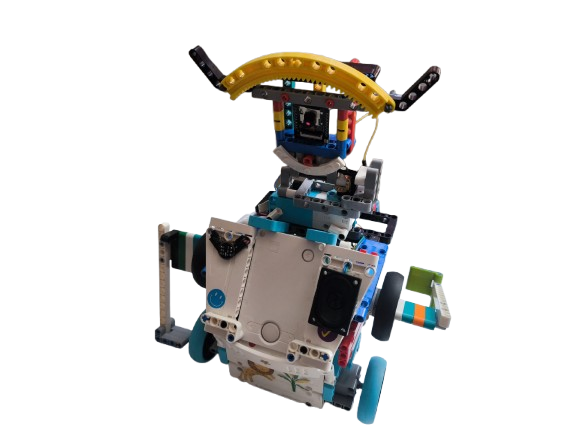
\includegraphics[width=\linewidth, height=0.32\textheight, keepaspectratio]{robot-trisense-perspectiva.png}
    \end{minipage}
    \hfill
    \begin{minipage}[b]{0.48\textwidth}
        \centering
        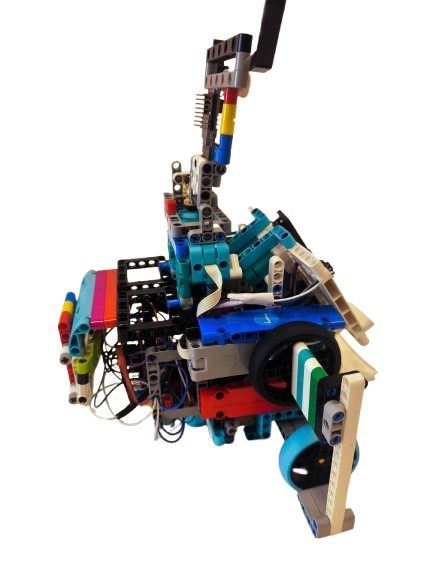
\includegraphics[width=\linewidth, height=0.32\textheight, keepaspectratio]{robot-trisense-lateral.png}
    \end{minipage}
    \caption[Robotul TriSense — vedere de ansamblu]{%
        Robotul TriSense în configurația finală: vedere frontal-oblică (stânga) și laterală (dreapta).%
        \par\smallskip
        {\small Se observă corpul LEGO, hub-ul montat frontal, roțile laterale, brațele mobile și modulele audio/video integrate.}%
    }
    \label{fig:robot-overview}
\end{figure}

Pe hub, programul \texttt{main.py} (Pybricks) are o structură deliberat simplă: o buclă care procesează mesajele LPF2 și citește butoanele. Toată „personalitatea” motorie — felul în care ridică brațele când se bucură, tremurul din rutina de \emph{meltdown}, ritmul lent al respirației — este codificată în rutine apelate prin coduri numerice. Rutina de \emph{meltdown} merită o mențiune: pune în scenă, stilizat și inofensiv, starea de criză din secțiunea~\ref{sec:meltdown}, după care robotul se „liniștește” prin rutina de respirație, modelând pentru copil o strategie concretă de autoreglare. Citirea butoanelor folosește \emph{debounce} software și transmite codul către ESP32 pe canalul \texttt{btn} (butonul stâng: copilul vrea să vorbească; butonul drept: fotografiază construcția).

Pe ESP32, programul \texttt{main\_robot.py} este componenta cu cele mai multe responsabilități simultane — client MQTT, punte LPF2, player audio și recorder — pe un microcontroler fără sistem de operare. Bucla principală este de aceea integral non-blocantă. Două probleme de implementare au fost instructive. Prima: \emph{redarea sacadată} a vocii, cauzată de debitul variabil al Wi-Fi-ului care golea buffer-ul DMA al interfeței I2S; soluția a fost un pre-buffer TCP de 32~KB plus un buffer DMA de aceeași dimensiune (valori găsite empiric), după care întreruperile au dispărut complet. A doua: \emph{stabilitatea legăturii LPF2} — hub-ul declară „senzorul” deconectat dacă nu primește răspuns la \texttt{pr.process()} în circa 40~ms, iar operațiile audio și de rețea sunt blocante prin natura lor; a fost nevoie de un set întreg de ajustări (felii audio dimensionate sub pragul de toleranță, I2S non-blocant, recepție TCP fragmentată, un \emph{ticker} LPF2 pe al doilea nucleu și ferestre de stabilizare după I2S), detaliate în anexa~\ref{an:cap:implementare}. După aplicarea lor, deconectările au dispărut chiar în scenariul cel mai solicitant: înregistrare de 5~s urmată imediat de redarea răspunsului, cu mișcări comandate între ele.

\section{Aplicația „creier” de pe PC}

Pachetul \texttt{trisense} concentrează logica de nivel înalt; punctul de intrare pentru modul vocal (\texttt{run\_voice\_dialog.py}) pornește serverul TCP de voce și instanțiază \texttt{TriSenseBrain}. La sosirea unei transcrieri, creierul parcurge o cascadă de decizii: verifică întâi starea curentă (dacă un joc e în desfășurare, intrarea se interpretează în contextul lui), apoi caută intenții explicite de acțiune sau de joc și, abia dacă niciun tipar nu se potrivește, trimite textul modelului conversațional Gemini, al cărui \emph{system prompt} fixează persona robotului: prietenos, răbdător, propoziții scurte, întotdeauna încurajator. Sinteza vocală (\texttt{tts\_engine.py}) folosește două motoare aduse la același format de ieșire — Google Cloud TTS și \texttt{edge-tts} — cu comutare automată la orice eroare a motorului principal, astfel încât robotul să nu rămână niciodată mut.

\section{Jocurile terapeutice}

Fiecare joc pornește de la un construct psihologic documentat și se sprijină pe o combinație diferită de capabilități ale sistemului. Tabelul~\ref{tab:jocuri} sintetizează repertoriul implementat; descrierea completă a fiecărui joc — fluxul tehnic și beneficiul terapeutic — este reluată în anexa~\ref{an:cap:implementare}.

\begin{table}[htb]
    \centering
    \caption{Repertoriul de activități terapeutice implementate în TriSense.}
    \label{tab:jocuri}
    \small
    \begin{tabular}{|>{\raggedright\arraybackslash}p{3.4cm}|>{\raggedright\arraybackslash}p{4.3cm}|>{\raggedright\arraybackslash}p{5.3cm}|}
        \hline
        \textbf{Activitate} & \textbf{Construct vizat} & \textbf{Capabilități folosite} \\
        \hline
        Ghicește emoția & recunoașterea și etichetarea emoțiilor & mișcare + expresie pe LED, voce, transcriere \\
        Urmează tiparul & memorie de lucru secvențială, imitație motorie & secvențe motorii, evaluare de către terapeut \\
        Build the Model & planificare vizuo-spațială (Turnul din Hanoi) & hub, butoane, cameră, viziune zero-shot \\
        Breathing Buddy & autoreglare emoțională, prevenirea meltdown-ului & rutină motorie + ghidaj vocal sincronizat \\
        Stop \& Go & control inhibitor (Go/No-Go) & matrice + lumină centrală, voce \\
        Categorii rapide & fluență semantică, acces lexical & lanț vocal, validare cu modelul de limbaj \\
        Estimarea timpului & percepția temporală & cronometru local, lanț vocal \\
        Povestea co-construită & organizare narativă, schimb de rând & model conversațional (persona de povestitor) \\
        Dansează cu mine & imitație motorie, coordonare, descărcare & rutină motorie (brațe + roți) \\
        \hline
    \end{tabular}
\end{table}

Cel mai complex joc este \textbf{Build the Model}, inspirat din proba Turnului din Hanoi, care leagă toate componentele — hub, voce, butoane, cameră și viziune. Are trei niveluri cu dificultate crescătoare (turn, piramidă, „robot”): la pornire, creierul afișează tiparul pe matrice (cu \texttt{keep\_display}) și publică descrierea-țintă pentru puntea de viziune; copilul construiește în ritmul lui și, când termină, apasă butonul drept, care declanșează captura. Verdictul lui Gemini Vision devine feedback vocal — felicitare și trecere la nivelul următor, sau încurajare și o descriere blândă a ceea ce mai lipsește. Faptul că validarea vine de la un robot, nu de la un adult, scoate din ecuație presiunea evaluării sociale.

\section{Componenta de vedere artificială și metricile de sesiune}
\label{sec:viziune}

Scriptul \texttt{vision\_esp32cam\_bridge.py} ascultă cererile de captură, preia imaginea JPEG de la ESP32-CAM, construiește promptul pentru Gemini Vision și publică verdictul structurat (potrivire booleană, scor de încredere, descrierea scenei). Abordarea \emph{zero-shot} — fără model antrenat, doar descrieri în limbaj natural — a funcționat surprinzător de bine, dar a cerut o calibrare iterativă: descrieri pe nivelul potrivit de detaliu (pentru „robot”, silueta de ansamblu, nu piesă cu piesă), instrucțiuni explicite de ignorare a mâinilor și a fundalului, și un prag de acceptare coborât de la 0,6 la 0,4 — valoare care acceptă toate construcțiile corecte din teste, respingând în continuare construcțiile greșite (scoruri tipic sub 0,25).

Modulul \texttt{metrics\_logger.py} înregistrează fiecare eveniment relevant (început/sfârșit de sesiune, fiecare joc cu nivel, încercări, reușită, durată, scor) în două formate paralele — CSV și JSONL — și generează automat, la final, un raport sumar per copil și per activitate. Fiecare raport poartă explicit mențiunea că datele susțin sesiuni de joc ghidate și nu constituie un test clinic validat — o delimitare la fel de importantă ca funcționalitatea însăși.

\chapter{Testare, evaluare și considerații etice}
\label{cap:evaluare}

\section{Metodologie și rezultate funcționale}

Sistemul a fost evaluat exclusiv pe hardware real, în condiții apropiate de utilizarea efectivă: robotul complet asamblat, ESP32-CAM poziționat către zona de construcție, un laptop în aceeași rețea Wi-Fi și brokerul Mosquitto local. Am urmărit trei dimensiuni — corectitudinea funcțională a celor trei fluxuri (comandă, voce, viziune), calitatea percepută a interacțiunii și acuratețea verificării vizuale — fiecare verigă fiind testată întâi izolat (cu scripturi dedicate în folderul \texttt{testare/}), apoi în lanț complet. Pe lângă testarea tehnică, structura jocurilor și felul în care robotul oferă feedback au fost discutate cu Marius și Andreea Lumpan, psihoterapeuți care practică LEGO-Based Therapy în România \cite{lumpanagerpres2025}; rolul lor nu a fost să „certifice” clinic sistemul, ci să filtreze deciziile de design prin experiență terapeutică reală.

Pe \emph{lanțul de comandă} (PC$\rightarrow$MQTT$\rightarrow$ESP32$\rightarrow$LPF2$\rightarrow$hub), comenzile s-au executat consistent, cu întârziere insesizabilă; canalul de butoane a funcționat fiabil după adăugarea mecanismului de \emph{debounce}. Pe \emph{lanțul vocal}, problema redării sacadate a fost rezolvată definitiv prin buffering — după mărirea pre-buffer-ului TCP și a buffer-ului DMA la 32~KB nu am mai înregistrat nicio întrerupere — iar latența totală a unui schimb, dominată de apelurile cloud, s-a situat tipic în câteva secunde, acoperită natural de faptul că robotul „se gândește”. Pe \emph{lanțul de viziune}, după calibrarea din secțiunea~\ref{sec:viziune}, toate construcțiile corecte au fost acceptate, iar cele greșite respinse cu scoruri net inferioare pragului (în jur de 0,2), marja dintre cele două categorii fiind suficient de largă încât pragul să nu fie sensibil la valoarea exactă.

\section{Date din sesiunile de joc}

Infrastructura de metrici a fost validată în sesiuni reale de joc cu un copil (consemnat sub prenumele David), desfășurate în mai--iunie 2026. Tabelul~\ref{tab:sesiuni} extrage câteva evenimente reprezentative.

\begin{table}[htb]
    \centering
    \caption{Evenimente extrase din jurnalul de metrici al sesiunilor de joc.}
    \label{tab:sesiuni}
    \begin{tabular}{|l|>{\raggedright\arraybackslash}p{6cm}|l|}
        \hline
        \textbf{Activitate} & \textbf{Eveniment înregistrat} & \textbf{Rezultat} \\
        \hline
        Guess the Emotion & emoția-țintă „happy”, răspuns detectat „happy” & reușit \\
        Dance with me & durată 12~s, implicare detectată & reușit \\
        Build the Model (niv. 1) & prima încercare, scor 0,20, durată 38~s & respins corect\textsuperscript{*} \\
        Sesiune completă & durată totală 21,1 minute & — \\
        \hline
    \end{tabular}

    \raggedright\footnotesize\textsuperscript{*} fotografie trimisă înainte de finalizarea construcției — sistemul a respins corect și a încurajat continuarea.
\end{table}

Dincolo de valorile individuale, sesiunile au confirmat două proprietăți de design. Întâi, rapoartele generate automat (text și JSON) sunt direct inteligibile pentru un adult fără pregătire tehnică. Apoi, mutarea controlului pe butoanele hub-ului a schimbat vizibil dinamica interacțiunii: copilul nu se mai uită la laptop, întreaga sesiune se desfășoară între el și robot.

\section{Limitări și considerații etice}

Evaluarea onestă impune consemnarea limitelor actuale: \textbf{dependența de internet} (dialogul, transcrierea și viziunea folosesc servicii cloud; offline, sistemul păstrează doar mișcările, animațiile și salutul pre-generat), \textbf{fereastra fixă de înregistrare} de 5~s (care poate trunchia enunțuri lungi — soluția corectă fiind detecția automată a sfârșitului vorbirii), \textbf{sensibilitatea viziunii} la iluminare slabă și încadrare parțială, și \textbf{evaluarea în mediu controlat} (sesiunile de test s-au desfășurat în mediu familiar, nu în cabinet; validarea cu copii neurodivergenți în context clinic real rămâne etapa următoare, condiționată de avizele etice).

Un sistem destinat copiilor neurodivergenți ridică obligații etice tratate ca parte din specificație: \textbf{fără pretenții de diagnostic} (TriSense este un instrument de suport în sesiuni ghidate de un adult, iar fiecare raport poartă explicit această mențiune); \textbf{terapeutul rămâne în control} (robotul propune activități, adultul decide continuarea, pauza sau oprirea); \textbf{protecția datelor} (numele copilului este stocat doar local, fotografiile sunt procesate punctual și nu arhivate, iar orice înregistrare a unei sesiuni reale necesită consimțământul informat al părinților, conform GDPR); și \textbf{proiectare pentru siguranță emoțională} (feedback exclusiv pozitiv, fără penalizare, cu pauze de respirație la semne de frustrare).

\chapter{Concluzii}
\label{cap:concluzii}

\section{Concluzii generale}

Lucrarea a pornit de la o întrebare pragmatică — se poate construi, din componente accesibile, un robot capabil să susțină activități terapeutice reale pentru copii neurodivergenți? — iar răspunsul demonstrat practic este afirmativ. TriSense există, funcționează cap-coadă pe hard\-ware real și acoperă un ciclu complet de interacțiune: copilul apasă un buton, vorbește, robotul îl înțelege, îi răspunde cu voce și mișcare, îi propune jocuri, îi verifică vizual construcțiile LEGO și consemnează totul pentru terapeut.

Din perspectivă tehnică, principala concluzie este că arhitectura distribuită pe trei niveluri — fiecare dispozitiv făcând strict ceea ce știe cel mai bine — a fost decizia care a făcut restul posibil: hub-ul LEGO nu știe că există internet, ESP32 nu știe ce spune modelul de limbaj, PC-ul nu atinge niciun motor. Această separare a făcut fiecare componentă testabilă izolat și a localizat imediat fiecare defect, de la redarea sacadată (rezolvată prin buffering) până la interferența modelului generativ cu logica jocului (rezolvată prin izolarea stărilor). Din perspectivă aplicativă, sistemul transpune fidel principiile din literatură: predictibilitatea și repetabilitatea care fac copilul disponibil pentru învățare \cite{scassellati2012, dautenhahn2004}, materialul LEGO intrinsec motivant \cite{legoff2004, owens2008}, feedback-ul imediat și exclusiv pozitiv, și rolul de mediator, nu de substitut. Merită consemnată și o concluzie metodologică: puterea modelelor generative vine la pachet cu nevoia de a le îngrădi explicit — prin prompturi atent formulate, praguri calibrate empiric și protejarea fluxului de control al jocurilor de creativitatea modelului conversațional.

\section{Direcții de dezvoltare ulterioară}

Câteva direcții se conturează natural: \textbf{validarea clinică extinsă} — primele sesiuni reale cu un copil neurodivergent au decurs încurajator, dar confirmarea eficacității cere un studiu amplu, cu protocol formal și avize etice, în colaborare cu terapeuți specializați în LBT; \textbf{completarea tripticului funcțiilor executive} cu jocurile aflate în stadiu de prototip (N-back verbal și Stroop adaptat); \textbf{detecția stării emoționale din voce} (analiza prozodiei, pentru a sesiza frustrarea înainte de escaladare); \textbf{înlocuirea ferestrei fixe de înregistrare} cu detecția automată a activității vocale; \textbf{funcționarea offline} prin modele locale; și o \textbf{interfață web pentru terapeut} (configurarea sesiunii, urmărirea în timp real, istoricul de metrici per copil).

Închei cu observația care mi se pare cea mai valoroasă din întregul proiect: niciuna dintre componentele folosite — setul LEGO, plăcile ESP32, serviciile de inteligență artificială — nu este exotică sau scumpă. Tot ce desparte un set educațional de un instrument terapeutic este integrarea. Iar integrarea, spre deosebire de hard\-ware-ul specializat, se poate replica oriunde există un calculator, o rețea Wi-Fi și cineva dispus să o facă.


\printbibliography[heading=bibintoc]

% Anexe (conțin materialul detaliat din varianta completă a lucrării)
\appendix

\chapter{Structura proiectului software}
\label{anexa:cod}

Codul sursă complet al sistemului este disponibil în repository-ul public al proiectului:

\begin{center}
    \url{https://github.com/DoublxB/Trisense}
\end{center}

Componentele principale sunt organizate astfel:

\begin{table}[htb]
    \centering
    \caption{Fișierele și modulele principale ale proiectului.}
    \label{tab:structura}
    \small
    \begin{tabular}{|l|l|}
        \hline
        \textbf{Fișier / modul} & \textbf{Rol} \\
        \hline
        \texttt{main.py} & firmware Pybricks pentru hub-ul LEGO \\
        \texttt{main\_robot.py} & firmware MicroPython pentru placa LMS-ESP32 \\
        \texttt{run\_voice\_dialog.py} & punct de intrare al creierului (mod vocal) \\
        \texttt{trisense/brain.py} & orchestrarea stărilor, dialogului și jocurilor \\
        \texttt{trisense/ai\_client.py} & interfața cu modelele Gemini (dialog, STT) \\
        \texttt{trisense/tts\_engine.py} & sinteza vocală cu fallback \\
        \texttt{trisense/cognitive\_games.py} & definițiile jocurilor și nivelurilor \\
        \texttt{trisense/mqtt\_layer.py} & stratul de comunicație MQTT \\
        \texttt{trisense/voice\_tcp\_server.py} & serverul TCP pentru audio de la robot \\
        \texttt{trisense/metrics\_logger.py} & jurnalizarea metricilor de sesiune \\
        \texttt{testare/vision\_esp32cam\_bridge.py} & puntea cameră--Gemini Vision \\
        \hline
    \end{tabular}
\end{table}

\chapter{Fundamente teoretice și studii de specialitate}
\label{an:cap:preliminarii}

Acest capitol trece în revistă literatura care a stat la baza proiectului — de la studiile clinice despre terapia bazată pe LEGO și despre interacțiunea copiilor cu autism cu roboții, la reperele constructiviste (Piaget) și socioculturale (Vygotsky), la poziționarea eclectică față de orientările psihologice majore (cognitiv-comportamentală și umanistă), până la conceptele și tehnologiile pe care se sprijină implementarea. Am încercat să păstrez un fir logic: pornesc de la întrebarea „de ce ar ajuta un robot un copil neurodivergent?”, continui cu „ce spun studiile și teoriile clasice că funcționează?” și închei cu „ce instrumente tehnice am la dispoziție ca să construiesc așa ceva?”.

\section{Neurodivergența: tulburările din spectrul autist și ADHD}

Termenul de \emph{neurodivergență} a apărut ca alternativă la limbajul strict medical și descrie variațiile naturale ale funcționării neurologice umane. În această categorie intră, printre altele, tulburările din spectrul autist (TSA), tulburarea de deficit de atenție și hiperactivitate (ADHD) și dislexia. Conform Manualului de Diagnostic și Statistică a Tulburărilor Mintale, ediția a cincea \cite{apa2013}, TSA se caracterizează prin deficite persistente în comunicarea și interacțiunea socială, alături de tipare restrictive și repetitive de comportament, interese sau activități. Severitatea variază enorm de la un copil la altul — de aici și denumirea de „spectru”.

Pentru lucrarea de față, două aspecte ale TSA sunt deosebit de relevante. Primul: copiii din spectru procesează adesea cu dificultate indiciile sociale subtile (expresii faciale, ton al vocii, contact vizual), ceea ce face interacțiunea cu alți oameni obositoare și uneori anxiogenă. Al doilea: aceiași copii răspund de regulă foarte bine la medii \emph{structurate și predictibile}, în care regulile sunt explicite și consecințele sunt consistente. Ambele observații conduc, după cum vom vedea, direct către robotică.

În cazul ADHD, dificultățile centrale țin de funcțiile executive — control inhibitor, memorie de lucru și flexibilitate cognitivă \cite{diamond2013} — competențe pe care le abordăm explicit, împreună cu rolul terapeutului uman în sesiune, în subsecțiunea~\ref{sec:executive-terapeut}.

\subsection{Suprasolicitarea senzorială și fenomenul de \emph{meltdown}}
\label{an:sec:meltdown}

Un fenomen aparte, central pentru orice intervenție adresată copiilor din spectru, este criza de suprasolicitare — în literatura de limbă engleză, \emph{meltdown}. Termenul este adesea confundat, în limbajul comun, cu „criza de nervi” sau cu capriciul. Distincția este însă esențială și bine documentată: capriciul este un comportament orientat către un scop (copilul urmărește să obțină ceva și se oprește când îl obține), pe când meltdown-ul este o reacție involuntară de descărcare, declanșată atunci când acumularea de stimuli — senzoriali, emoționali, cognitivi — depășește capacitatea de procesare a copilului. Odată depășit acest prag, copilul nu mai are acces la mecanismele obișnuite de autoreglare: nu „alege” să se comporte astfel și, în consecință, nici recompensele, nici admonestările nu au efect în acel moment — dimpotrivă, presiunea suplimentară prelungește episodul.

Cercetarea clinică susține această lectură. Mazefsky și colaboratorii \cite{mazefsky2013} argumentează că dificultățile de reglare emoțională nu sunt un simptom periferic al TSA, ci un mecanism central care explică o mare parte din comportamentele-problemă observate: copilul din spectru resimte emoțiile la intensitate crescută, dar dispune de strategii de reglare mai puține și mai fragile, astfel încât stări pe care un copil neurotipic le-ar „metaboliza” discret pot escalada rapid. O perspectivă complementară, valoroasă tocmai pentru că vine din interior, o oferă Phung și colaboratorii \cite{phung2021}, care au intervievat adolescenți autiști despre propriile experiențe: tinerii descriu meltdown-ul ca pe o pierdere a controlului precedată de semne care se acumulează treptat (iritabilitate, nevoia de retragere, hipersensibilitate la zgomot) și urmată de epuizare și, frecvent, de rușine. Două concluzii practice se desprind din aceste relatări: episoadele pot fi adesea \emph{prevenite} dacă semnele timpurii sunt observate la timp, iar reacția cea mai utilă a celor din jur este una calmă, predictibilă și lipsită de judecată.

Aceste observații au modelat TriSense pe două planuri. Pe plan \emph{preventiv}, întreaga interacțiune este construită să reducă riscul de suprasolicitare: structura sesiunilor este predictibilă, feedback-ul este întotdeauna pozitiv, iar exercițiul de respirație ghidat de robot oferă o pauză de reglare exact în logica pauzelor senzoriale recomandate în practica terapeutică. Pe plan \emph{educativ}, robotul poate interpreta el însuși, în scenarii demonstrative, o variantă stilizată și inofensivă a stării de criză — brațe agitate, expresie tulburată pe matricea de LED-uri (figura~\ref{fig:robot}) — după care „se liniștește” prin propria rutină de respirație. Copilul ajunge astfel să observe și să denumească starea din exterior, fără să fie el cel aflat în ea, iar robotul modelează în același timp o strategie concretă de autoreglare. Este aceeași logică a externalizării pe care o folosesc poveștile sociale ale lui Gray, despre care va fi vorba mai jos.

\section{Terapia bazată pe LEGO}

Punctul de plecare conceptual al proiectului TriSense este terapia bazată pe LEGO (LEGO-Based Therapy, prescurtat LBT). Ideea îi aparține doctorului Daniel LeGoff, neuropsiholog clinician, care a observat în sala de așteptare a cabinetului său ceva neașteptat: doi copii cu autism, care în mod obișnuit nu inițiau interacțiuni sociale, au început spontan să vorbească unul cu altul despre construcțiile LEGO pe care le aduseseră de acasă. Pornind de la această observație, LeGoff a formalizat un protocol de intervenție în care construcția colaborativă cu piese LEGO devine mediul terapeutic propriu-zis \cite{legoff2004}.

În studiul inițial, publicat în \emph{Journal of Autism and Developmental Disorders}, LeGoff a urmărit 47 de copii cu diagnostic din spectrul autist pe parcursul a 24 de săptămâni de terapie. Rezultatele au arătat îmbunătățiri semnificative pe trei dimensiuni măsurate: frecvența autoinițierii contactului social, durata interacțiunilor sociale și reducerea comportamentelor stereotipe. Un studiu ulterior de follow-up pe trei ani \cite{legoff2006} a confirmat că efectele se mențin în timp și că progresul copiilor din grupul LBT a depășit semnificativ grupul de control care primise alte intervenții.

Independent de echipa lui LeGoff, grupul lui Simon Baron-Cohen de la Universitatea Cambridge a comparat LBT cu un alt program consacrat de abilități sociale (Social Use of Language Programme) pe copii cu autism înalt funcțional și sindrom Asperger \cite{owens2008}. Concluzia: copiii din grupul LEGO au înregistrat ameliorări superioare ale comportamentelor sociale specifice autismului. Autorii atribuie acest efect caracterului \emph{intrinsec motivant} al materialului — copiii nu „fac terapie”, ci se joacă cu LEGO, iar abilitățile sociale se exersează ca efect secundar al jocului.

De ce funcționează piesele LEGO atât de bine? Literatura oferă câteva explicații convergente. Sistemul LEGO este predictibil: piesele se îmbină într-un singur mod corect, regulile sunt fizice, nu sociale, iar rezultatul este vizibil imediat. Pentru un copil căruia ambiguitatea socială îi provoacă anxietate, acest determinism este eliberator. În plus, construcția după model implică exact funcțiile executive vizate de intervențiile cognitive: planificare, memorie de lucru, atenție la detaliu și persistență la sarcină.

TriSense preia acest cadru și îl augmentează: robotul devine partenerul de joc care propune modelul, urmărește construcția și oferă feedback — un rol pe care în LBT clasic îl joacă terapeutul sau un alt copil.

În România, metoda a fost adaptată de psihoterapeuții Marius și Andreea Lumpan, care descriu LBT ca pe un cadru în care copiii neurodivergenți și neurotipici construiesc împreună, dezvoltând competențe emoționale, sociale și cognitive \cite{lumpanagerpres2025}. Experiența mea alături de ei în acest context a completat lectura articolelor internaționale: am observat direct cum terapeutul calibrează ritmul sesiunii, când intervine înainte de escaladare și cum materialul LEGO menține copilul în sarcină fără presiune evaluativă — observații care au influențat ulterior designul jocurilor TriSense.

\section{Constructivism cognitiv și învățarea socioculturală}

Pe lângă protocoalele clinice și studiile despre roboți, designul activităților TriSense se sprijină și pe două orientări clasice din psihologia educațională: constructivismul lui Jean Piaget și teoria socioculturală a lui Lev Vygotsky. Nu le folosim ca etichete teoretice goale — explică de ce are sens ca un copil să \emph{construiască} cu mâinile, să primească indicii clare și să dialogheze cu un partener predictibil.

Piaget descrie dezvoltarea ca pe un proces activ: copilul nu absoarbe pasiv informații, ci își construiește înțelegerea prin acțiune asupra mediului, prin asimilarea experiențelor noi în scheme deja existente și prin acomodare când realitatea nu se potrivește așteptărilor \cite{piaget1969}. Manipularea pieselor LEGO — potrivirea, ordinea, verificarea dacă modelul arată „ca pe ecran” — este un exemplu concret de învățare prin acțiune: copilul formulează o ipoteză (reproduc structura), o testează (apasă butonul de verificare), primește feedback și ajustează construcția. Jocul „Build the Model”, imitarea tiparelor de mișcare sau sortarea cuvintelor pe categorii se aliniază acestei logici: sarcina solicită organizare, seriere și persistență, nu memorarea mecanică a unui răspuns dat de adult.

Vygotsky mută accentul de la individ izolat la \emph{medierea socială}. Învățarea semnificativă apare în zona dintre ce poate copilul singur și ce poate cu sprijin — zona proximală de dezvoltare —, iar un partener mai competent (profesor, părinte, coleg) structurează sarcina pas cu pas, apoi retrage treptat ajutorul \cite{vygotsky1978}. Limbajul, gesturile și semnele culturale (inclusiv reprezentări vizuale simple) sunt instrumente prin care copilul internalizează strategii pe care inițial le folosește doar cu ajutor. TriSense se plasează în acest cadru ca \emph{mediator}: robotul nu înlocuiește terapeutul, dar oferă scaffolding consecvent — instrucțiuni scurte, același ritual de salut, feedback fără pedeapsă, nivele de dificultate crescătoare la construcții, dialog ghidat în povestea co-construită. Predictibilitatea robotului reduce încărcătura socială ambiguă, astfel încât copilul să poată lucra în zona proximală: face el pasul, dar nu rămâne singur cu confuzia.

Cele două perspective nu se exclud. Piaget explică de ce contează materialul concret și eșecul constructiv (construcția care nu se potrivește); Vygotsky explică de ce contează partenerul, vocea și structura socială a jocului. TriSense le combină: LEGO ca mediu de acțiune, robotul ca partener de scaffolding, adultul din cameră ca reper uman — în linie cu ideea, documentată și în literatura despre roboți, că prezența unui mediator mecanic poate facilita, nu bloca, interacțiunea cu oamenii. Menținem aceeași limită ca în restul capitolului: activitățile sunt exerciții de suport inspirate din teorie, nu evaluări de stadiu piagetian sau intervenții clinice validate în sens strict.

\subsection{Funcții executive, consistență robotică și rolul terapeutului uman}
\label{sec:executive-terapeut}

În cazul ADHD, dificultățile centrale țin de funcțiile executive: control inhibitor, memorie de lucru și flexibilitate cognitivă \cite{diamond2013}. Diamond arată că aceste trei funcții de bază se pot antrena prin exerciții repetate, gradate ca dificultate — exact tipul de activitate pe care un sistem robotic îl poate administra cu o consecvență pe care un om nu o poate garanta sesiune după sesiune. Jocuri precum Stop \& Go (control inhibitor), estimarea timpului sau construcția după model solicită aceleași competențe, într-un cadru ludic, cu reguli explicite și feedback imediat.

Avantajul robotului este tocmai regularitatea: aceleași instrucțiuni, același ritm, aceeași reacție la reușită sau la eșec. Limitarea este la fel de clară: robotul nu \emph{simte} oboseala copilului, nu citește nuanțele unei voci obosite sau ale unei frustrări care se acumulează înainte de meltdown, nu adaptează empatic tonul în funcție de starea afectivă a momentului. Aici intervine colaborarea cu terapeutul uman — psiholog, terapeut ocupațional sau educator specializat — care conduce sesiunea, observă semnele timpurii de suprasolicitare și decide când se continuă, când se face pauză sau când se schimbă activitatea.

TriSense este gândit explicit în această logică de \emph{complementaritate}, nu de înlocuire. Robotul structurează jocul, oferă feedback consecvent și înregistrează metrici obiective (durate, încercări, reușite) pe care terapeutul le poate folosi la evaluare; terapeutul rămâne cel care aduce relația, intuiția clinică și sensibilitatea la emoțiile copilului. Definirea activităților și a constrângerilor etice din proiect a fost discutată cu Marius și Andreea Lumpan, psihoterapeuți cu experiență în practica LBT din România \cite{lumpanagerpres2025} — nu ca validare clinică a sistemului, ci ca verificare că jocurile rămân blânde, predictibile și utile într-un context ghidat de adult. Raportul de sesiune generat automat este un instrument de sprijin pentru terapeut, nu un substitut al observației directe.

\subsection{Orientări psihologice și poziționarea TriSense}
\label{sec:orientari-psihologice}

Pe lângă constructivism și teoria socioculturală, designul TriSense se raportează la cele trei mari orientări istorice ale psihologiei: psihanaliza, behaviorismul și umanismul. Proiectul nu aparține unei singure școli — este deliberat eclectic. Jocurile care antrenează funcțiile executive (Stop \& Go, construcții gradate, fluență semantică) se sprijină pe logica cognitiv-comportamentală: practică repetată, feedback imediat, întărire pozitivă \cite{diamond2013}. Aceste instrumente au sens atunci când copilul este disponibil pentru sarcină și toleranța la frustrare nu este deja depășită.

În schimb, modul în care abordăm suprasolicitarea senzorială și meltdown-ul (secțiunea~\ref{an:sec:meltdown}) urmează o orientare umanistă. Rogers descrie relația terapeutică ca pe un cadru de acceptare necondiționată, în care persoana nu este redusă la un set de comportamente corectabile \cite{rogers1951}. Relatările adolescenților autiști despre meltdown confirmă miza acestei poziții: episoadele sunt adesea urmate de rușine, iar presiunea, pedeapsa sau expunerea publică le prelungesc sau le agravează \cite{phung2021}. De aceea, în momentul crizei recompensele și admonestările nu au efect — iar robotul nu „sancționează” eșecul; scenariile de criză sunt stilizate, voluntare și urmate de reglare (respirație ghidată), sub supravegherea unui adult care poate simți starea copilului și adapta tonul.

Tensiunea dintre antrenarea cognitivă și respectul pentru experiența subiectivă nu este un defect al proiectului, ci o alegere de design: robotul aduce consistența necesară exercițiilor structurate; terapeutul uman aduce empatia, intuiția și decizia de oprire — complementaritate deja descrisă în subsecțiunea~\ref{sec:executive-terapeut}. Nu am ales o teorie ca etichetă decorativă; am distins ce se potrivește fiecărei situații din sesiune.

\section{Robotica asistivă în intervențiile pentru copii cu autism}

\subsection{De ce roboți?}

Întrebarea pare legitimă: dacă dificultățile copiilor cu TSA sunt de natură socială, de ce am introduce în terapie o mașină, în loc să exersăm direct interacțiunea umană? Literatura de specialitate a documentat însă un fenomen consistent: mulți copii cu autism interacționează mai ușor cu roboții decât cu oamenii, cel puțin în fazele inițiale ale intervenției.

Explicația ține de natura stimulului social. Interacțiunea umană este copleșitoare informațional — fețe care se schimbă permanent, intonații variabile, reguli sociale implicite. Un robot, în schimb, este \emph{simplu, predictibil și răbdător}: repetă aceeași acțiune identic de fiecare dată, nu se plictisește, nu judecă și nu transmite semnale sociale ambigue. Dautenhahn și Werry, pionierii proiectului AURORA (unul dintre primele programe de cercetare dedicate roboților ca instrumente terapeutice pentru copii cu autism), au argumentat încă din 2004 că tocmai această simplitate controlabilă face din robot un mediator ideal: un pas intermediar între lumea predictibilă a obiectelor și lumea impredictibilă a oamenilor \cite{dautenhahn2004}.

\subsection{Ce arată studiile}

Domeniul s-a maturizat rapid, iar mai multe sinteze sistematice permit astăzi o imagine de ansamblu. Scassellati, Admoni și Matarić \cite{scassellati2012}, într-o trecere în revistă publicată în \emph{Annual Review of Biomedical Engineering}, documentează că în prezența roboților copiii cu TSA manifestă comportamente sociale pe care le afișează rar în alte contexte: contact vizual prelungit, atenție comună, imitație spontană și inițierea interacțiunii. La fel de important, autorii observă că aceste comportamente nu rămân direcționate exclusiv către robot — în multe studii ele se extind către adulții prezenți în încăpere, ceea ce sugerează un potențial real de transfer.

Robins și colaboratorii \cite{robins2005}, lucrând cu robotul umanoid minimalist KASPAR, au arătat în studii longitudinale că expunerea repetată la un robot cu comportament simplu și repetitiv crește treptat disponibilitatea copiilor de a interacționa — întâi cu robotul, apoi cu experimentatorul uman. Robotul a funcționat, în termenii autorilor, ca \emph{mediator social}: obiectul comun de interes care face posibilă interacțiunea triadică copil–robot–adult.

Kim și colaboratorii \cite{kim2013} au adus o contribuție metodologică importantă: într-un experiment controlat, copiii cu TSA au vorbit mai mult cu un adult în prezența unui robot decât în prezența unui alt adult sau a unui joc pe tabletă. Cu alte cuvinte, robotul nu doar atrage atenția copilului, ci funcționează ca întăritor („embedded reinforcer”) al comportamentului social îndreptat către oameni.

Sintezele critice mai recente impun însă și prudență. Diehl și colaboratorii \cite{diehl2012} notează că multe studii din domeniu au eșantioane mici și design exploratoriu, iar Pennisi și colaboratorii \cite{pennisi2016}, într-o sinteză sistematică, confirmă rezultatele pozitive privind implicarea și reducerea comportamentelor repetitive, dar subliniază nevoia de studii clinice riguroase. Cabibihan și colaboratorii \cite{cabibihan2013} oferă o taxonomie utilă a rolurilor pe care un robot le poate juca în terapie — partener de joc, model comportamental, instrument de evaluare, mediator social — și a caracteristicilor de design care contează: aspect non-amenințător, comportament repetabil, feedback imediat. Ricks și Colton \cite{ricks2010} adaugă o observație de design relevantă pentru TriSense: roboții cu aspect mecanic, non-umanoid, sunt adesea mai bine primiți de copiii cu TSA decât cei cu aspect uman realist, care pot genera disconfort.

Poziționarea TriSense față de această literatură este directă: sistemul nostru este un robot non-umanoid construit din piese LEGO (material deja familiar și pozitiv conotat pentru copil), care joacă rolul de partener de joc și mediator, administrează activități inspirate din LBT și din probele clasice de funcții executive și produce metrici obiective pentru terapeut — fără nicio pretenție de diagnostic.

\subsection{Funcțiile executive și jocurile cognitive}

Mai multe activități din TriSense sunt inspirate din probe consacrate în neuropsihologie, adaptate în formă de joc. Jocul „Build the Model” pornește de la \emph{Turnul din Hanoi}, o probă clasică de planificare vizuo-spațială: copilul trebuie să reproducă o structură-țintă respectând o ordine de asamblare, ceea ce solicită memoria de lucru și planificarea pas-cu-pas. „Stop \& Go” preia paradigma Go/No-Go (control inhibitor), exercițiul de estimare a timpului pornește de la probele de percepție temporală (legate de planificare și de impulsivitate), iar „categoriile rapide” adaptează probele de fluență semantică (acces lexical). Jocurile aflate încă în stadiu de prototip preiau paradigmele N-back (actualizarea memoriei de lucru) și Stroop (inhibiția interferenței). Toate aceste funcții sunt discutate pe larg de Diamond \cite{diamond2013} ca fiind antrenabile prin practică repetată.

Este esențial de subliniat statutul acestor activități: ele sunt \emph{exerciții terapeutice inspirate din procedee standard, nu teste clinice validate}. TriSense nu măsoară inteligența și nu diagnostichează — înregistrează doar indicatori de joc (durate, încercări, reușite) pe care terapeutul îi poate interpreta în context.

\subsection{Rutina și predictibilitatea: Social Stories}

Un ultim reper conceptual vine din metoda \emph{Social Stories} a lui Carol Gray \cite{gray2010}: scenarii sociale scurte, formulate identic la fiecare repetare, care pregătesc copilul pentru situații sociale concrete. TriSense aplică același principiu în structura sesiunilor — salutul, formulele de încurajare și ritualul de încheiere folosesc formulări consecvente, astfel încât copilul să știe mereu la ce să se aștepte.

\section{Sisteme cyber-fizice}

Un \emph{sistem cyber-fizic} (Cyber-Physical System, CPS) integrează strâns calculul, comunicația și procesele fizice: senzorii și actuatorii interacționează cu mediul, în timp ce componenta de calcul — adesea distribuită pe mai multe dispozitive — monitorizează și controlează aceste procese în buclă închisă \cite{lee2008}. Lee subliniază că provocarea centrală a unui CPS nu este puterea de calcul, ci \emph{orchestrarea}: sincronizarea în timp real a unor componente diferite, cu cerințe de fiabilitate pe care software-ul clasic de birou nu le are.

TriSense este un CPS în sens deplin. Bucla sa de control percepe starea fizică a lumii (vocea copilului prin microfon, construcția LEGO prin cameră, apăsările de buton de pe hub), o procesează printr-o componentă de calcul distribuită pe trei dispozitive plus servicii cloud și o transformă înapoi în acțiuni fizice: mișcări ale brațelor, animații pe matricea de LED-uri, vorbire sintetizată redată pe difuzor. Caracterul \emph{adaptiv} vine din stratul de inteligență artificială: răspunsurile verbale se generează dinamic în funcție de contextul conversației și de starea jocului, iar verificarea construcțiilor tolerează variații de poziționare, iluminare și perspectivă.

\section{Platformele hardware utilizate}

\subsection{LEGO SPIKE Prime și firmware-ul Pybricks}

LEGO\textsuperscript{®} SPIKE\texttrademark{} Prime este o platformă educațională construită în jurul unui hub programabil cu șase porturi de motoare/senzori, o matrice de LED-uri $5\times5$, butoane fizice și baterie proprie. Alegerea ei nu a fost întâmplătoare: pentru un copil care face deja terapie LEGO, un robot construit din LEGO nu este un obiect străin, ci o extensie a unui univers familiar.

În locul firmware-ului oficial am folosit \emph{Pybricks} \cite{pybricks}, un firmware open-source bazat pe MicroPython. Decizia a fost dictată de două nevoi pe care mediul oficial nu le acoperă: control fin, neîntrerupt, asupra motoarelor și matricei de LED-uri, și — esențial pentru arhitectura noastră — acces programabil la portul LPF2, prin care hub-ul poate comunica cu dispozitive externe ca și cum ar fi senzori LEGO.

\subsection{Placa LMS-ESP32}

LMS-ESP32 \cite{antonsmindstorms} este o placă de extensie construită în jurul microcontrolerului ESP32, proiectată specific pentru a se conecta la portul LPF2 al hub-urilor LEGO. Din punctul de vedere al hub-ului, placa se prezintă ca un senzor LEGO obișnuit; în realitate, ea aduce tot ce îi lipsește hub-ului: conectivitate Wi-Fi, interfață audio I2S și putere de calcul suplimentară. Pe placă rulează MicroPython \cite{micropython}, iar în TriSense ea joacă rolul de „trunchi cerebral”: leagă corpul LEGO de rețea și de creierul de pe PC.

Lanțul audio al robotului este construit în jurul acestei plăci: un amplificator MAX98357A cu difuzor de 4~$\Omega$ pentru voce (interfața I2S pe pinii GPIO 14/15/26, cu activare pe GPIO~32) și un microfon digital INMP441 (date pe GPIO~33, cu ceasurile partajate cu amplificatorul).

\subsection{Modulul ESP32-CAM}

Pentru componenta de vedere artificială am folosit un modul ESP32-CAM AI-Thinker — o cameră de cost foarte redus (sub 50 de lei) cu server HTTP propriu. Modulul este alimentat din placa LMS-ESP32, dar comunică independent prin Wi-Fi: PC-ul îi cere o imagine JPEG printr-o simplă cerere HTTP la endpoint-ul \texttt{/capture}. Această decuplare s-a dovedit valoroasă în practică — camera poate fi poziționată liber față de robot, oriunde încadrează bine zona de construcție.

\section{Protocoale și tehnologii de comunicație}

\subsection{MQTT}

MQTT \cite{mqtt} este un protocol de mesagerie de tip \emph{publish/subscribe} proiectat pentru dispozitive cu resurse limitate — exact profilul plăcii ESP32. Un broker central (în implementarea noastră, Mosquitto, rulat local pe PC) intermediază mesajele: fiecare participant publică pe topicuri și se abonează la topicurile care îl interesează, fără să cunoască direct ceilalți participanți. Această decuplare simplifică mult arhitectura: creierul de pe PC, robotul și puntea de viziune comunică toate prin broker, iar căderea temporară a unei componente nu blochează restul sistemului.

\subsection{LPF2 și biblioteca PupRemote}

LPF2 (LEGO Power Functions 2) este protocolul serial proprietar prin care hub-urile LEGO comunică cu senzorii. Biblioteca \emph{PupRemote} \cite{pupremote} construiește peste LPF2 un mecanism de „comenzi cu nume”: definești pe ambele capete un canal cu un format de date, iar biblioteca se ocupă de serializare și de handshake-ul de senzor. TriSense folosește două canale: \texttt{cmd}, prin care ESP32 trimite hub-ului coduri numerice de acțiune, și \texttt{btn}, adăugat în sens invers, prin care hub-ul raportează apăsările butoanelor fizice.

\subsection{Streaming audio prin TCP}

MQTT este potrivit pentru mesaje scurte, nu pentru fluxuri audio. Pentru voce am folosit conexiuni TCP directe între PC și ESP32: pe portul 8765 robotul trimite către PC audio brut de la microfon (pentru transcriere), iar pe portul 8766 PC-ul trimite către robot vocea sintetizată (PCM mono, 16 biți, 24~kHz), redată pe difuzor prin I2S. Alegerea formatului PCM necomprimat a fost deliberată: decodarea unui format comprimat ar fi depășit resursele plăcii, în timp ce lățimea de bandă a unei rețele locale acoperă fără probleme debitul de 48~KB/s al fluxului.

\section{Serviciile de inteligență artificială}

\subsection{Modele de limbaj de mari dimensiuni}

Componenta conversațională folosește modelele Google Gemini \cite{gemini}. Comportamentul modelului este constrâns printr-un \emph{system prompt} dedicat, care impune un ton cald și răbdător, propoziții scurte, vocabular adecvat vârstei și — important în context terapeutic — evitarea oricăror formulări care ar putea suna a evaluare sau critică. Tot prin prompt, modelul este instruit să recunoască intențiile de joc exprimate liber de copil („I want to build something!”) și să le semnaleze sistemului.

\subsection{Transcrierea vorbirii și sinteza vocală}

Lanțul vocal complet are trei verigi. Transcrierea (speech-to-text) se face tot cu Gemini, căruia i se trimite înregistrarea audio împreună cu instrucțiuni de transcriere fidelă. Generarea răspunsului revine modelului conversațional. Sinteza vocală (text-to-speech) folosește două motoare cu comutare automată: Google Cloud TTS cu vocea neurală \texttt{en-US-Neural2-F} ca motor principal și \texttt{edge-tts} cu vocea \texttt{en-US-JennyNeural} ca alternativă — ambele producând voci feminine calde, alese deliberat pentru contextul interacțiunii cu copii.

\subsection{Vedere artificială multimodală}

Pentru verificarea construcțiilor LEGO am ales o abordare care merită o justificare: în loc să antrenăm un clasificator de imagini dedicat (care ar fi cerut sute de fotografii etichetate pentru fiecare model și ar fi fost rigid la schimbarea modelelor), folosim modelul multimodal Gemini Vision în regim \emph{zero-shot}. Modelul primește fotografia construcției și o descriere în limbaj natural a țintei („un turn din patru cuburi portocalii 2$\times$4, așezate unul peste altul”) și întoarce un verdict structurat: potrivire da/nu, scor de încredere și o descriere a ceea ce vede. Adăugarea unui model nou în joc se reduce astfel la scrierea unui paragraf descriptiv — fără date de antrenare, fără reantrenare.

\include{anexa-3-arhitectura}
\include{anexa-4-implementare}
\chapter{Testare, evaluare și considerații etice}
\label{an:cap:evaluare}

\section{Metodologia de testare}

Sistemul a fost evaluat exclusiv pe hardware real, în condiții cât mai apropiate de utilizarea efectivă: robotul complet asamblat, modulul ESP32-CAM poziționat către zona de construcție, un laptop în aceeași rețea Wi-Fi și brokerul Mosquitto rulând local. Am urmărit trei dimensiuni:

\begin{enumerate}
    \item \textbf{corectitudinea funcțională} a celor trei fluxuri (comandă, voce, viziune) — fiecare verigă testată întâi izolat, apoi în lanț complet;
    \item \textbf{calitatea percepută a interacțiunii} — continuitatea redării vocale, timpul de la apăsarea butonului până la răspunsul robotului, stabilitatea legăturii hub--ESP32;
    \item \textbf{acuratețea verificării vizuale} a construcțiilor LEGO pe cele trei modele ale jocului.
\end{enumerate}

Pentru fiecare componentă hardware există scripturi de test dedicate în folderul \texttt{testare/} (ton de probă pe difuzor, nivel de semnal pe microfon, comenzi MQTT individuale), care au permis izolarea rapidă a problemelor — o practică ce s-a dovedit indispensabilă într-un sistem cu atâtea puncte de defectare posibile.

Pe lângă testarea tehnică, am urmărit și o validare calitativă a ideii de intervenție. Structura jocurilor și felul în care robotul oferă feedback au fost discutate cu Marius și Andreea Lumpan, psihoterapeuți care practică LEGO-Based Therapy în România \cite{lumpanagerpres2025}. Rolul lor nu a fost să „certifice” clinic sistemul — lucru care ar cere un protocol separat și un eșantion de copii — ci să filtreze deciziile de design prin experiență terapeutică reală: cât de lungă poate fi o instrucțiune, când devine un feedback prea evaluativ, de ce e mai bine să spui „mai încearcă o dată” decât „greșit” și de ce pauzele de reglare trebuie să apară înainte ca frustrarea să escaladeze.

\section{Rezultate funcționale}

\subsection{Lanțul de comandă}

Pe traseul PC $\rightarrow$ MQTT $\rightarrow$ ESP32 $\rightarrow$ LPF2 $\rightarrow$ hub, comenzile de mișcare și animațiile s-au executat consistent, cu o întârziere insesizabilă pentru utilizator. Canalul invers, de butoane, a funcționat fiabil după adăugarea mecanismului de \emph{debounce} pe hub; fără el, o singură apăsare genera ocazional evenimente duplicate. Stabilitatea legăturii LPF2 a impus o disciplină strictă în firmware-ul ESP32 — orice operație blocantă mai lungă de câteva sute de milisecunde ducea la desincronizarea handshake-ului cu hub-ul, motiv pentru care toate operațiile de rețea au fost rescrise non-blocant.

\subsection{Lanțul vocal}

Problema redării sacadate, descrisă în capitolul~\ref{an:cap:implementare}, a fost rezolvată definitiv prin buffering: după mărirea pre-buffer-ului TCP și a buffer-ului DMA la 32~KB, nu am mai înregistrat nicio întrerupere de redare pe parcursul tuturor sesiunilor ulterioare. Latența totală a unui schimb conversațional — de la sfârșitul celor 5 secunde de înregistrare până la începutul răspunsului vocal al robotului — este dominată de apelurile către serviciile cloud (transcriere, generare, sinteză) și s-a situat tipic în intervalul de câteva secunde; pentru copil, așteptarea este acoperită natural de faptul că robotul „se gândește”. Transcrierea înregistrărilor s-a dovedit suficient de precisă pentru detectarea fiabilă a intențiilor de joc, inclusiv la vorbire nenativă.

\subsection{Lanțul de viziune}

Cele trei modele ale jocului „Build the Model” au fost testate cu construcții corecte și greșite, în condiții variate de încadrare. După calibrarea descrisă în secțiunea~\ref{an:sec:viziune} (simplificarea descrierii pentru modelul „robot” și coborârea pragului la 0,4), toate construcțiile corecte au fost acceptate, iar cele greșite — de exemplu, fotografia trimisă înainte de terminarea turnului — au fost respinse cu scoruri net inferioare pragului (în jur de 0,2). Marja dintre scorurile construcțiilor corecte și ale celor greșite s-a dovedit suficient de largă încât pragul să nu fie sensibil la alegerea exactă a valorii.

\section{Date din sesiunile de joc}

Infrastructura de metrici a fost validată în sesiuni reale de joc cu un copil (consemnat în rapoarte sub prenumele David), desfășurate în mai--iunie 2026. Tabelul~\ref{an:tab:sesiuni} extrage câteva evenimente reprezentative din jurnalul de metrici.

\begin{table}[htb]
    \centering
    \caption{Evenimente extrase din jurnalul de metrici al sesiunilor de joc.}
    \label{an:tab:sesiuni}
    \begin{tabular}{|l|>{\raggedright\arraybackslash}p{6cm}|l|}
        \hline
        \textbf{Activitate} & \textbf{Eveniment înregistrat} & \textbf{Rezultat} \\
        \hline
        Guess the Emotion & emoția-țintă „happy”, răspuns detectat „happy” & reușit \\
        Dance with me & durată 12~s, implicare detectată & reușit \\
        Build the Model (niv. 1) & prima încercare, scor 0,20, durată 38~s & respins corect\textsuperscript{*} \\
        Sesiune completă & durată totală 21,1 minute & — \\
        \hline
    \end{tabular}

    \raggedright\footnotesize\textsuperscript{*} fotografie trimisă înainte de finalizarea construcției — sistemul a respins corect și a încurajat continuarea.
\end{table}

Dincolo de valorile individuale, sesiunile au confirmat două proprietăți de design. Întâi, rapoartele generate automat (text și JSON) sunt direct inteligibile pentru un adult fără pregătire tehnică — durata sesiunii, jocurile jucate și rezultatele apar în limbaj natural. Apoi, mutarea controlului pe butoanele hub-ului a schimbat vizibil dinamica interacțiunii: copilul nu se mai uită la laptop, întreaga sesiune se desfășoară între el și robot.

\section{Limitări}

Evaluarea onestă a sistemului impune consemnarea limitelor lui actuale:

\begin{itemize}
    \item \textbf{dependența de internet}: dialogul, transcrierea și viziunea folosesc servicii cloud; fără conexiune, sistemul păstrează doar mișcările, animațiile și salutul pre-generat;
    \item \textbf{fereastra fixă de înregistrare}: cele 5 secunde de captură vocală pot trunchia enunțuri mai lungi; detecția automată a sfârșitului vorbirii (VAD) ar fi soluția corectă;
    \item \textbf{sensibilitatea viziunii la condiții}: iluminarea slabă și încadrarea parțială a construcției degradează scorurile de încredere;
    \item \textbf{evaluarea în mediu controlat}: sesiunile de test s-au desfășurat în mediu familiar, nu în cabinet terapeutic; validarea cu copii neurodivergenți în context clinic real rămâne etapa următoare și este condiționată de avizele etice corespunzătoare.
\end{itemize}

\section{Considerații etice}

Un sistem destinat copiilor neurodivergenți ridică obligații etice pe care le-am tratat ca parte din specificație, nu ca formalitate:

\begin{itemize}
    \item \textbf{fără pretenții de diagnostic}: TriSense este un instrument de \emph{suport} în sesiuni ghidate de un adult; activitățile sunt exerciții inspirate din procedee standard, nu teste clinice validate, iar fiecare raport de sesiune poartă explicit această mențiune;
    \item \textbf{terapeutul rămâne în control}: robotul nu ia decizii terapeutice — propune activități, iar adultul prezent decide continuarea, pauza sau oprirea;
    \item \textbf{protecția datelor}: numele copilului este stocat doar local, pe calculatorul terapeutului; fotografiile construcțiilor sunt procesate punctual pentru verificare și nu sunt arhivate; orice înregistrare audio sau video a unei sesiuni cu un copil real necesită consimțământul informat, scris, al părinților sau tutorilor, conform GDPR;
    \item \textbf{proiectare pentru siguranță emoțională}: feedback-ul este exclusiv pozitiv, eșecurile declanșează încurajare și niciodată penalizare, iar sistemul propune pauze de respirație la semne de frustrare — prevenirea suprasolicitării senzoriale a fost un criteriu de design, nu o opțiune.
\end{itemize}


\end{document}
